% Options for packages loaded elsewhere
\PassOptionsToPackage{unicode}{hyperref}
\PassOptionsToPackage{hyphens}{url}
%
\documentclass[
  ignorenonframetext,
]{beamer}
\usepackage{pgfpages}
\setbeamertemplate{caption}[numbered]
\setbeamertemplate{caption label separator}{: }
\setbeamercolor{caption name}{fg=normal text.fg}
\beamertemplatenavigationsymbolsempty
% Prevent slide breaks in the middle of a paragraph
\widowpenalties 1 10000
\raggedbottom
\setbeamertemplate{part page}{
  \centering
  \begin{beamercolorbox}[sep=16pt,center]{part title}
    \usebeamerfont{part title}\insertpart\par
  \end{beamercolorbox}
}
\setbeamertemplate{section page}{
  \centering
  \begin{beamercolorbox}[sep=12pt,center]{part title}
    \usebeamerfont{section title}\insertsection\par
  \end{beamercolorbox}
}
\setbeamertemplate{subsection page}{
  \centering
  \begin{beamercolorbox}[sep=8pt,center]{part title}
    \usebeamerfont{subsection title}\insertsubsection\par
  \end{beamercolorbox}
}
\AtBeginPart{
  \frame{\partpage}
}
\AtBeginSection{
  \ifbibliography
  \else
    \frame{\sectionpage}
  \fi
}
\AtBeginSubsection{
  \frame{\subsectionpage}
}
\usepackage{lmodern}
\usepackage{amssymb,amsmath}
\usepackage{ifxetex,ifluatex}
\ifnum 0\ifxetex 1\fi\ifluatex 1\fi=0 % if pdftex
  \usepackage[T1]{fontenc}
  \usepackage[utf8]{inputenc}
  \usepackage{textcomp} % provide euro and other symbols
\else % if luatex or xetex
  \usepackage{unicode-math}
  \defaultfontfeatures{Scale=MatchLowercase}
  \defaultfontfeatures[\rmfamily]{Ligatures=TeX,Scale=1}
\fi
% Use upquote if available, for straight quotes in verbatim environments
\IfFileExists{upquote.sty}{\usepackage{upquote}}{}
\IfFileExists{microtype.sty}{% use microtype if available
  \usepackage[]{microtype}
  \UseMicrotypeSet[protrusion]{basicmath} % disable protrusion for tt fonts
}{}
\makeatletter
\@ifundefined{KOMAClassName}{% if non-KOMA class
  \IfFileExists{parskip.sty}{%
    \usepackage{parskip}
  }{% else
    \setlength{\parindent}{0pt}
    \setlength{\parskip}{6pt plus 2pt minus 1pt}}
}{% if KOMA class
  \KOMAoptions{parskip=half}}
\makeatother
\usepackage{xcolor}
\IfFileExists{xurl.sty}{\usepackage{xurl}}{} % add URL line breaks if available
\IfFileExists{bookmark.sty}{\usepackage{bookmark}}{\usepackage{hyperref}}
\hypersetup{
  pdftitle={Initial results},
  hidelinks,
  pdfcreator={LaTeX via pandoc}}
\urlstyle{same} % disable monospaced font for URLs
\newif\ifbibliography
\setlength{\emergencystretch}{3em} % prevent overfull lines
\providecommand{\tightlist}{%
  \setlength{\itemsep}{0pt}\setlength{\parskip}{0pt}}
\setcounter{secnumdepth}{-\maxdimen} % remove section numbering

\title{Initial results}
\date{}

\begin{document}
\frame{\titlepage}

\begin{frame}{Species abundance distributions}
\protect\hypertarget{species-abundance-distributions}{}

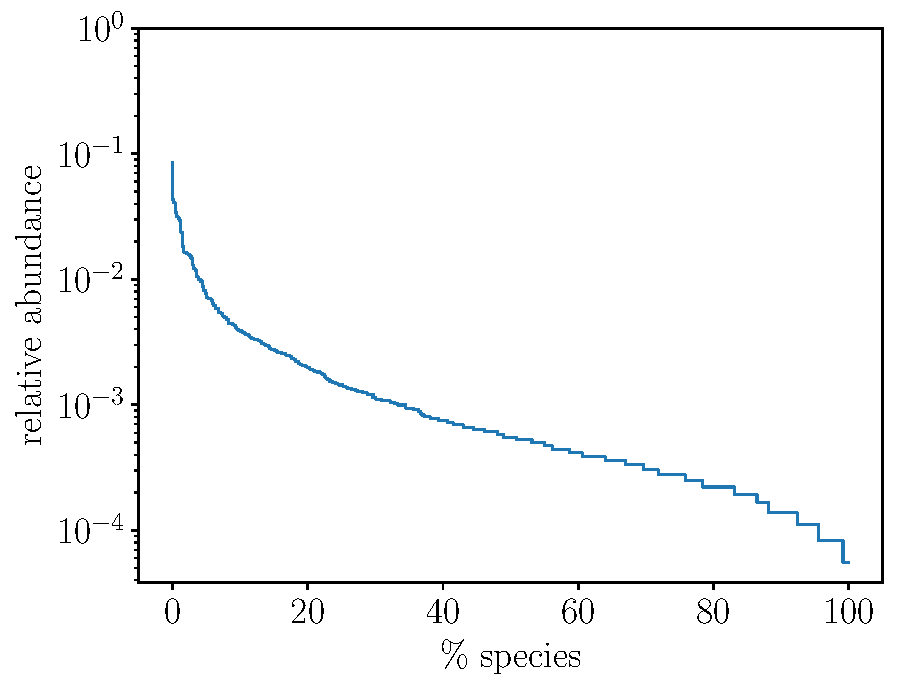
\includegraphics[width=\linewidth]{figs/species_abundance_curve_0.pdf}

\end{frame}

\begin{frame}{Species abundance distributions}
\protect\hypertarget{species-abundance-distributions-1}{}

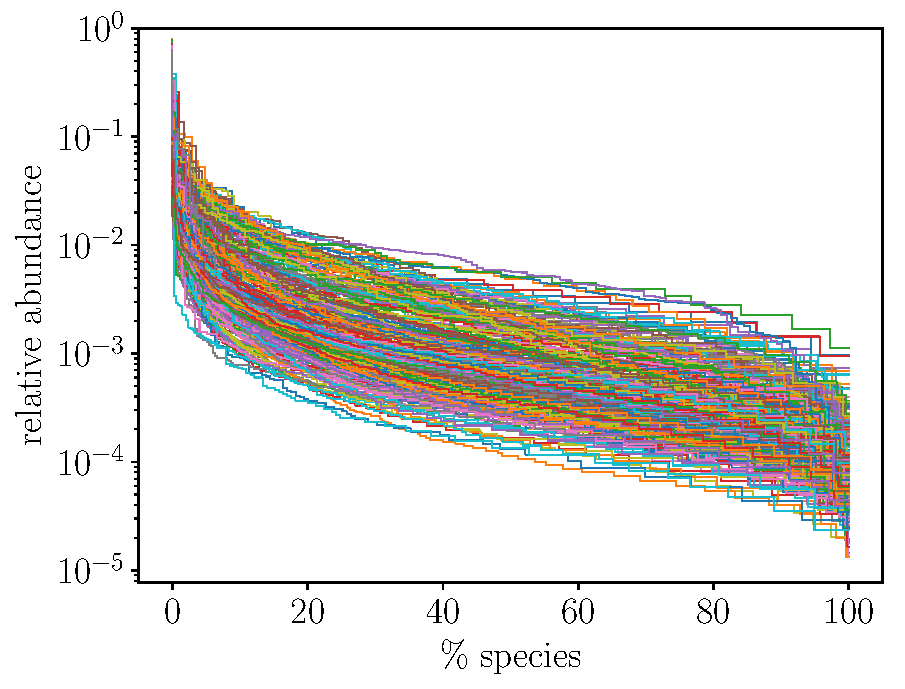
\includegraphics[width=\linewidth]{figs/species_abundance_curve_4.pdf}

\end{frame}

\begin{frame}{Species abundance distributions with lognormal curve}
\protect\hypertarget{species-abundance-distributions-with-lognormal-curve}{}

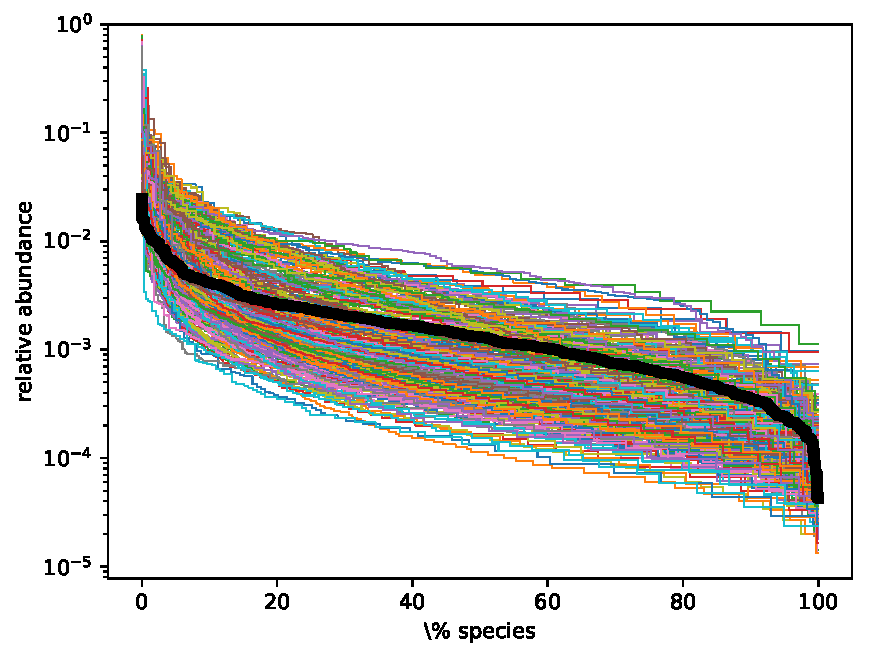
\includegraphics[width=\linewidth]{figs/species_abundance_curve_5.pdf}

\end{frame}

\begin{frame}{Shannon diversity}
\protect\hypertarget{shannon-diversity}{}

\Large The Shannon diversity \(S\) is defined
\[S = -\sum_{i=1}^N p_i \ln(p_i).\]

\normalsize

\(\implies\) maximum for \(y_i = 1/N\) for all \(i\)

\(\implies\) minimum for \(y_i = 1\), \(y_j = 0\) for \(j \neq i\)

(one of many metrics for ``diversity'' of a population)

\end{frame}

\begin{frame}{Shannon diversity}
\protect\hypertarget{shannon-diversity-1}{}

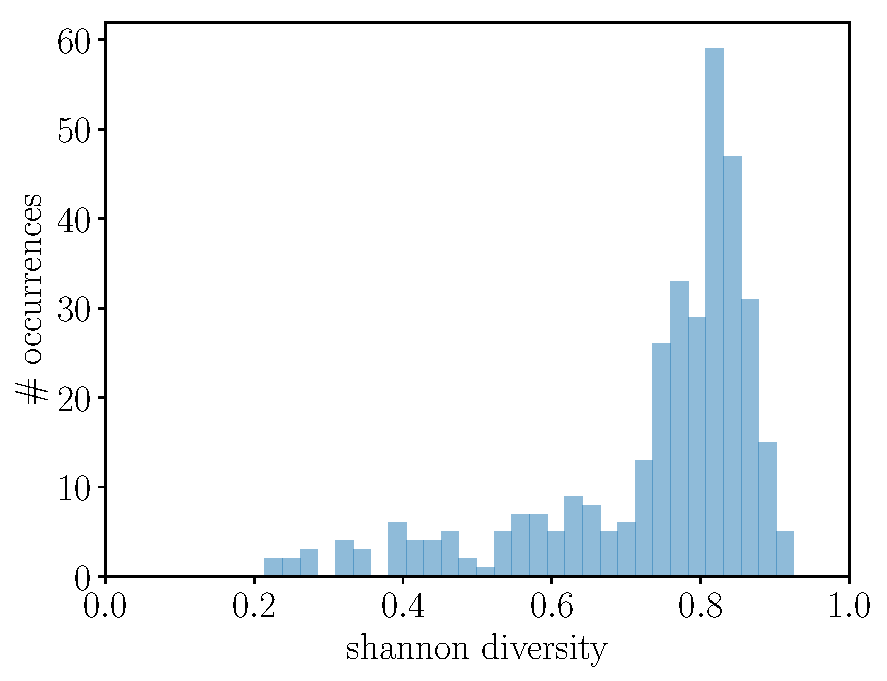
\includegraphics[width=\linewidth]{figs/shannon_div_0}

\end{frame}

\begin{frame}{Shannon diversity with lognormal distribution}
\protect\hypertarget{shannon-diversity-with-lognormal-distribution}{}

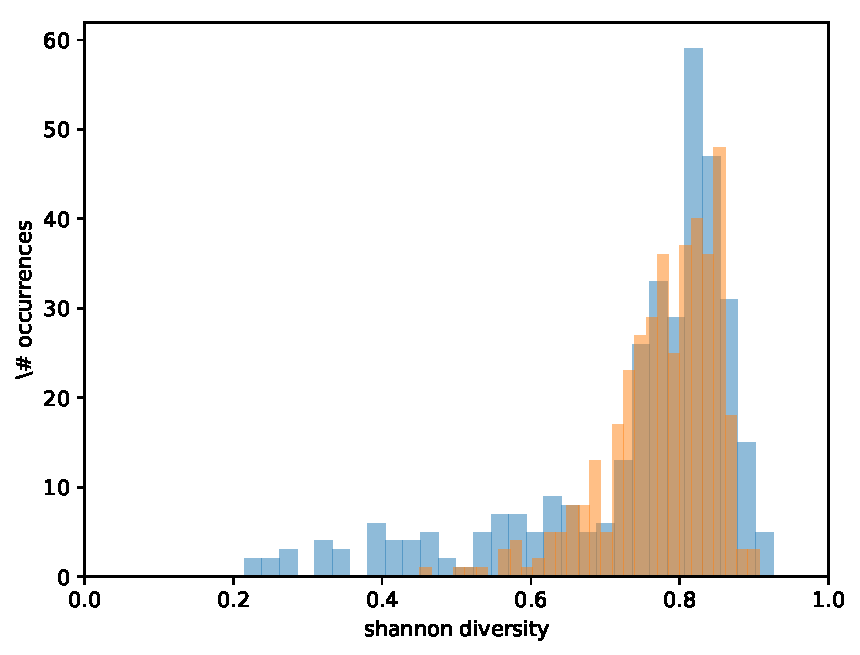
\includegraphics[width=\linewidth]{figs/shannon_div_1}

\end{frame}

\begin{frame}{Unifrac\footnote{image from mothur.org/w/images/5/5b/UnweightedUniFracMeasure.jpg}}
\protect\hypertarget{unifrac}{}

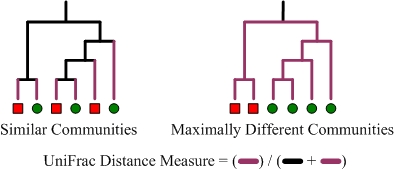
\includegraphics[width=\linewidth]{figs/UnweightedUniFracMeasure.jpg}

\end{frame}

\begin{frame}{Unifrac distance matrix (weighted)}
\protect\hypertarget{unifrac-distance-matrix-weighted}{}

\centering

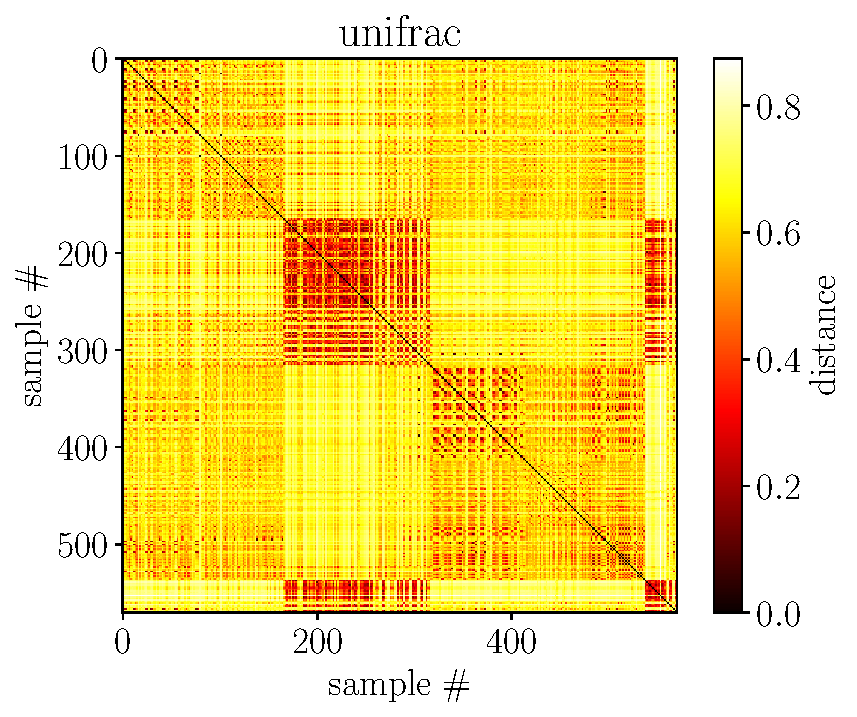
\includegraphics[width=.9\linewidth]{figs/unifrac_distance_matrix}

\end{frame}

\begin{frame}{Unifrac distance matrix (unweighted)}
\protect\hypertarget{unifrac-distance-matrix-unweighted}{}

\centering

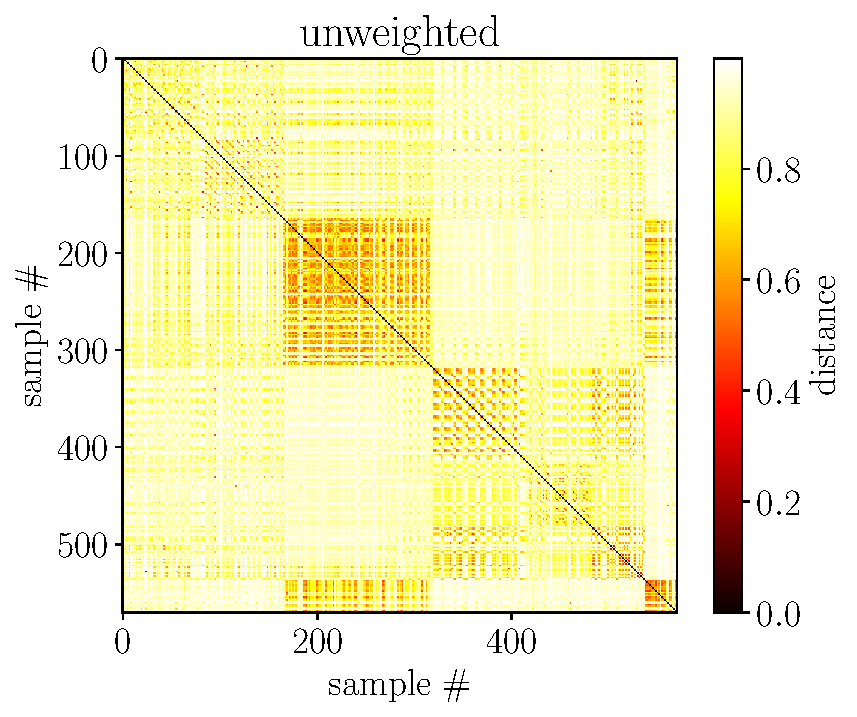
\includegraphics[width=.9\linewidth]{figs/unweighted_distance_matrix}

\end{frame}

\begin{frame}{\(L_2\)-norm distance matrix (weighted)}
\protect\hypertarget{l_2-norm-distance-matrix-weighted}{}

\centering

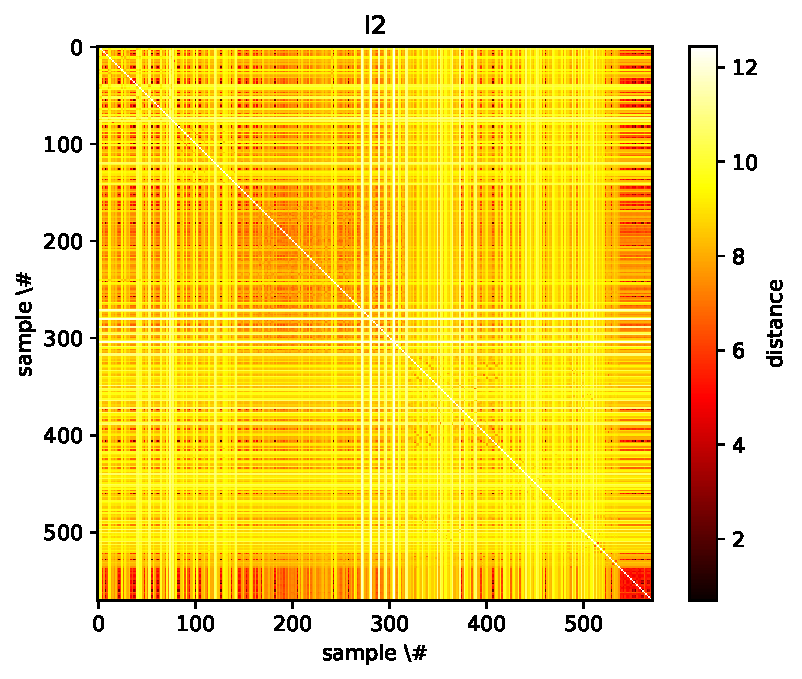
\includegraphics[width=.9\linewidth]{figs/l2_distance_matrix}

\end{frame}

\begin{frame}{Future work?}
\protect\hypertarget{future-work}{}

\Large

\begin{itemize}
\tightlist
\item
  Estimate size of available microbiome pool (species abundance curve)
\item
  Coarse-grain at different taxonomic resolutions
\item
  Include metadata analyses
\item
  How can we address nestedness?
\end{itemize}

\end{frame}

\end{document}
